% Options for packages loaded elsewhere
\PassOptionsToPackage{unicode}{hyperref}
\PassOptionsToPackage{hyphens}{url}
\PassOptionsToPackage{dvipsnames,svgnames,x11names}{xcolor}
%
\documentclass[
  letterpaper,
  DIV=11,
  numbers=noendperiod]{scrreprt}

\usepackage{amsmath,amssymb}
\usepackage{iftex}
\ifPDFTeX
  \usepackage[T1]{fontenc}
  \usepackage[utf8]{inputenc}
  \usepackage{textcomp} % provide euro and other symbols
\else % if luatex or xetex
  \usepackage{unicode-math}
  \defaultfontfeatures{Scale=MatchLowercase}
  \defaultfontfeatures[\rmfamily]{Ligatures=TeX,Scale=1}
\fi
\usepackage{lmodern}
\ifPDFTeX\else  
    % xetex/luatex font selection
\fi
% Use upquote if available, for straight quotes in verbatim environments
\IfFileExists{upquote.sty}{\usepackage{upquote}}{}
\IfFileExists{microtype.sty}{% use microtype if available
  \usepackage[]{microtype}
  \UseMicrotypeSet[protrusion]{basicmath} % disable protrusion for tt fonts
}{}
\makeatletter
\@ifundefined{KOMAClassName}{% if non-KOMA class
  \IfFileExists{parskip.sty}{%
    \usepackage{parskip}
  }{% else
    \setlength{\parindent}{0pt}
    \setlength{\parskip}{6pt plus 2pt minus 1pt}}
}{% if KOMA class
  \KOMAoptions{parskip=half}}
\makeatother
\usepackage{xcolor}
\setlength{\emergencystretch}{3em} % prevent overfull lines
\setcounter{secnumdepth}{5}
% Make \paragraph and \subparagraph free-standing
\ifx\paragraph\undefined\else
  \let\oldparagraph\paragraph
  \renewcommand{\paragraph}[1]{\oldparagraph{#1}\mbox{}}
\fi
\ifx\subparagraph\undefined\else
  \let\oldsubparagraph\subparagraph
  \renewcommand{\subparagraph}[1]{\oldsubparagraph{#1}\mbox{}}
\fi


\providecommand{\tightlist}{%
  \setlength{\itemsep}{0pt}\setlength{\parskip}{0pt}}\usepackage{longtable,booktabs,array}
\usepackage{calc} % for calculating minipage widths
% Correct order of tables after \paragraph or \subparagraph
\usepackage{etoolbox}
\makeatletter
\patchcmd\longtable{\par}{\if@noskipsec\mbox{}\fi\par}{}{}
\makeatother
% Allow footnotes in longtable head/foot
\IfFileExists{footnotehyper.sty}{\usepackage{footnotehyper}}{\usepackage{footnote}}
\makesavenoteenv{longtable}
\usepackage{graphicx}
\makeatletter
\def\maxwidth{\ifdim\Gin@nat@width>\linewidth\linewidth\else\Gin@nat@width\fi}
\def\maxheight{\ifdim\Gin@nat@height>\textheight\textheight\else\Gin@nat@height\fi}
\makeatother
% Scale images if necessary, so that they will not overflow the page
% margins by default, and it is still possible to overwrite the defaults
% using explicit options in \includegraphics[width, height, ...]{}
\setkeys{Gin}{width=\maxwidth,height=\maxheight,keepaspectratio}
% Set default figure placement to htbp
\makeatletter
\def\fps@figure{htbp}
\makeatother
\newlength{\cslhangindent}
\setlength{\cslhangindent}{1.5em}
\newlength{\csllabelwidth}
\setlength{\csllabelwidth}{3em}
\newlength{\cslentryspacingunit} % times entry-spacing
\setlength{\cslentryspacingunit}{\parskip}
\newenvironment{CSLReferences}[2] % #1 hanging-ident, #2 entry spacing
 {% don't indent paragraphs
  \setlength{\parindent}{0pt}
  % turn on hanging indent if param 1 is 1
  \ifodd #1
  \let\oldpar\par
  \def\par{\hangindent=\cslhangindent\oldpar}
  \fi
  % set entry spacing
  \setlength{\parskip}{#2\cslentryspacingunit}
 }%
 {}
\usepackage{calc}
\newcommand{\CSLBlock}[1]{#1\hfill\break}
\newcommand{\CSLLeftMargin}[1]{\parbox[t]{\csllabelwidth}{#1}}
\newcommand{\CSLRightInline}[1]{\parbox[t]{\linewidth - \csllabelwidth}{#1}\break}
\newcommand{\CSLIndent}[1]{\hspace{\cslhangindent}#1}

\KOMAoption{captions}{tableheading}
\makeatletter
\makeatother
\makeatletter
\@ifpackageloaded{bookmark}{}{\usepackage{bookmark}}
\makeatother
\makeatletter
\@ifpackageloaded{caption}{}{\usepackage{caption}}
\AtBeginDocument{%
\ifdefined\contentsname
  \renewcommand*\contentsname{Table of contents}
\else
  \newcommand\contentsname{Table of contents}
\fi
\ifdefined\listfigurename
  \renewcommand*\listfigurename{List of Figures}
\else
  \newcommand\listfigurename{List of Figures}
\fi
\ifdefined\listtablename
  \renewcommand*\listtablename{List of Tables}
\else
  \newcommand\listtablename{List of Tables}
\fi
\ifdefined\figurename
  \renewcommand*\figurename{Figure}
\else
  \newcommand\figurename{Figure}
\fi
\ifdefined\tablename
  \renewcommand*\tablename{Table}
\else
  \newcommand\tablename{Table}
\fi
}
\@ifpackageloaded{float}{}{\usepackage{float}}
\floatstyle{ruled}
\@ifundefined{c@chapter}{\newfloat{codelisting}{h}{lop}}{\newfloat{codelisting}{h}{lop}[chapter]}
\floatname{codelisting}{Listing}
\newcommand*\listoflistings{\listof{codelisting}{List of Listings}}
\makeatother
\makeatletter
\@ifpackageloaded{caption}{}{\usepackage{caption}}
\@ifpackageloaded{subcaption}{}{\usepackage{subcaption}}
\makeatother
\makeatletter
\@ifpackageloaded{tcolorbox}{}{\usepackage[skins,breakable]{tcolorbox}}
\makeatother
\makeatletter
\@ifundefined{shadecolor}{\definecolor{shadecolor}{rgb}{.97, .97, .97}}
\makeatother
\makeatletter
\makeatother
\makeatletter
\makeatother
\ifLuaTeX
  \usepackage{selnolig}  % disable illegal ligatures
\fi
\IfFileExists{bookmark.sty}{\usepackage{bookmark}}{\usepackage{hyperref}}
\IfFileExists{xurl.sty}{\usepackage{xurl}}{} % add URL line breaks if available
\urlstyle{same} % disable monospaced font for URLs
\hypersetup{
  colorlinks=true,
  linkcolor={blue},
  filecolor={Maroon},
  citecolor={Blue},
  urlcolor={Blue},
  pdfcreator={LaTeX via pandoc}}

\author{}
\date{2023-06-05}

\begin{document}
\ifdefined\Shaded\renewenvironment{Shaded}{\begin{tcolorbox}[enhanced, sharp corners, borderline west={3pt}{0pt}{shadecolor}, boxrule=0pt, frame hidden, interior hidden, breakable]}{\end{tcolorbox}}\fi

\renewcommand*\contentsname{Table of contents}
{
\hypersetup{linkcolor=}
\setcounter{tocdepth}{2}
\tableofcontents
}
\bookmarksetup{startatroot}

\hypertarget{our-vision-of-open-science}{%
\chapter*{Our vision of Open Science}\label{our-vision-of-open-science}}
\addcontentsline{toc}{chapter}{Our vision of Open Science}

\markboth{Our vision of Open Science}{Our vision of Open Science}

The core mission of ICArEHB is to build an integrative understanding of
human behavior in prehistoric times and assure that the main outputs of
this research are new and outstanding knowledge, ideas, and
understanding in the fields of prehistoric archaeology and human
evolution, that can be shared with other scientists and with the
society.

Particularly, the destructive nature of archaeology means that we must
stick to the highest standards; we must leave a maximum of elements
available for other scientists and the future generation of
archaeologists. To keep these standards, ICArEHB embraces the concept of
Open Science, i.e., research that is transparent and allows
reproducibility, the best guarantee to stay at the forefront. It means
that, as much as possible, our research projects are validated by our
peers before we start it, our procedures, software, and code, are made
accessible to others, and our results are shared with various audiences
(e.g., other scientists, the general public, policymakers) and our data
are archived for the future.

\hypertarget{open-methodologies}{%
\subsection*{Open methodologies}\label{open-methodologies}}
\addcontentsline{toc}{subsection}{Open methodologies}

Did you know that even before it starts, projects can be examined and
validated by other experts? This is the case for all projects funded in
ICArEHB, which go through peer review either by the third-party funder
or by an internal review process.

In addition, we encourage our researchers to pre-register their study in
journals and platforms allowing this format. This ensures that our study
plans are robust and helps to reduce the bias of publication, so all
results are shared, even if less exciting than expected.

\hypertarget{open-source}{%
\subsection*{Open source}\label{open-source}}
\addcontentsline{toc}{subsection}{Open source}

As much as possible, we use open-source software and file formats that
everyone can use. When we write code, or new software and apps, we
publish them and assure that they are available for the rest of the
community. Check out some of these examples here and here.

\hypertarget{open-publications}{%
\subsection*{Open publications}\label{open-publications}}
\addcontentsline{toc}{subsection}{Open publications}

Our scientific outputs are published in the form of articles,
monographs, handbooks, etc., privileging those platforms that will make
our research most visible to our peers, the scientific community, and
the general public.

In ICArEHB, all articles led by our integrated researchers are in Open
Access on the journal website or on the platform of publication. This
means that we prefer to pay to make sure that everyone can have access
to our production instead of asking the readers to pay. You can consult
our list of publications and respective links here.~

\hypertarget{open-communication}{%
\subsection*{Open communication}\label{open-communication}}
\addcontentsline{toc}{subsection}{Open communication}

Scientific publication is not a piece of cake, especially if you are not
used to it. In ICArEHB, we make a special effort to share our results
and our conclusions with other parts of society, with adapted media. The
Science Communication Lab is dedicated to inventing new formats and
producing content for our outreach actions.~

Check here our past and future events of outreach. If you would like
ICArEHB to participate in school activities or in a fair, please contact
us to discuss possibilities.

We exchange updates on good practices in archaeology through our
collaboration with the company of contractual archaeology ERA
Arqueologia.

We also make special efforts to transform scientific work into policy
when necessary.

\hypertarget{open-data}{%
\subsection*{Open data}\label{open-data}}
\addcontentsline{toc}{subsection}{Open data}

Publications and communications are just the tip of the iceberg when it
comes to research, and the text, tables, and images that we publish are
just elements of a frontpage advertisement to the many hours of
recording, processing, and analysis of what is one of the most valuable
ICArEHB's contributions to the world: our data!

Factual data is the cornerstone of science, and access to data is
crucial in fully understanding and extending the work of others.
Providing free and general access to our data is the most effective way
of ensuring that the fruits of the research can be accessed, read, and
used as the basis for further research.

Bringing together the current demands of funding agencies with our will
to transform the way people share archaeological data, ICArEHB offers a
series of \protect\hyperlink{guidelines}{guidelines} to researchers, so
they can assess the open science level of a specific study, publication,
or project.

This guide tries to tackle most of the current demands for open science.
It is built around the use of trusted platforms that can support our
researchers throughout their entire project lifecycle, centralizing as
much as possible the different parts of the process, including
Preregistrations, Data Storage and Versioning, Pre-prints, License
attribution, Persistent Identifier Creation, Metadata creation for
maximum machine-actionable Findability, Accessibility, Interoperability,
and Re-usability (FAIR).

\bookmarksetup{startatroot}

\hypertarget{guidelines}{%
\chapter*{Guidelines}\label{guidelines}}
\addcontentsline{toc}{chapter}{Guidelines}

\markboth{Guidelines}{Guidelines}

Use the following criteria to guide and ``evaluate'' the Open Science
level of a specific study (when available, follow the links for wiki
pages on each topic). Most links point to the \href{www.osf.io}{Open
Science Framework}, but other trusted platforms are available.

\hypertarget{preparing-the-study}{%
\section*{Preparing the study}\label{preparing-the-study}}
\addcontentsline{toc}{section}{Preparing the study}

\markright{Preparing the study}

\hypertarget{pre-registration}{%
\subsubsection*{\texorpdfstring{\protect\hyperlink{pre-registration-1}{1.
Pre-registration}}{1. Pre-registration}}\label{pre-registration}}
\addcontentsline{toc}{subsubsection}{\protect\hyperlink{pre-registration-1}{1.
Pre-registration}}

Write a pre-registration or registered report and upload it on
\href{https://osf.io/registries}{OSF Registries}

\hypertarget{data-management-plan}{%
\subsubsection*{\texorpdfstring{\protect\hyperlink{data-management-plan-dmp}{2.
Data Management
Plan}}{2. Data Management Plan}}\label{data-management-plan}}
\addcontentsline{toc}{subsubsection}{\protect\hyperlink{data-management-plan-dmp}{2.
Data Management Plan}}

Check/write a data management plan (DMP)

\hypertarget{conducting-the-study}{%
\section*{Conducting the study}\label{conducting-the-study}}
\addcontentsline{toc}{section}{Conducting the study}

\markright{Conducting the study}

\hypertarget{data-collection-protocols}{%
\subsubsection*{\texorpdfstring{\protect\hyperlink{data-collection-protocols-1}{3.
Data collection
protocols}}{3. Data collection protocols}}\label{data-collection-protocols}}
\addcontentsline{toc}{subsubsection}{\protect\hyperlink{data-collection-protocols-1}{3.
Data collection protocols}}

Use and store understandable and accessible protocols for data
collection, including protocols for participant contact, participant
instructions, and data handling.

\hypertarget{data-dictionary}{%
\subsubsection*{\texorpdfstring{\protect\hyperlink{data-dictionary-1}{4.
Data dictionary}}{4. Data dictionary}}\label{data-dictionary}}
\addcontentsline{toc}{subsubsection}{\protect\hyperlink{data-dictionary-1}{4.
Data dictionary}}

Keep a codebook that gives an overview all the different measures and
the exact content of data files. This includes information like variable
names and labels, measurement levels and values. This can be a template
at first and be updated it if changes occur.

\hypertarget{logbook}{%
\subsubsection*{\texorpdfstring{\protect\hyperlink{logbook-1}{5.
Logbook}}{5. Logbook}}\label{logbook}}
\addcontentsline{toc}{subsubsection}{\protect\hyperlink{logbook-1}{5.
Logbook}}

Keep a logbook of all important events that occur during data collection

\hypertarget{data-storage}{%
\subsubsection*{\texorpdfstring{\protect\hyperlink{data-storage-1}{6.
Data storage}}{6. Data storage}}\label{data-storage}}
\addcontentsline{toc}{subsubsection}{\protect\hyperlink{data-storage-1}{6.
Data storage}}

Store your data logically and in a safe place from day 1

\hypertarget{scripts}{%
\subsubsection*{\texorpdfstring{\protect\hyperlink{scripts-1}{7.
Scripts}}{7. Scripts}}\label{scripts}}
\addcontentsline{toc}{subsubsection}{\protect\hyperlink{scripts-1}{7.
Scripts}}

Use understandable and accessible scripts/syntax for data analyses

\hypertarget{metadata}{%
\subsubsection*{\texorpdfstring{\protect\hyperlink{metadata-1}{8.
Metadata}}{8. Metadata}}\label{metadata}}
\addcontentsline{toc}{subsubsection}{\protect\hyperlink{metadata-1}{8.
Metadata}}

Use understandable and accessible Readme to describe research metadata.

\hypertarget{writing-the-manuscript}{%
\section*{Writing the manuscript}\label{writing-the-manuscript}}
\addcontentsline{toc}{section}{Writing the manuscript}

\markright{Writing the manuscript}

\hypertarget{version-control}{%
\subsubsection*{\texorpdfstring{\protect\hyperlink{version-control-1}{9.
Version control}}{9. Version control}}\label{version-control}}
\addcontentsline{toc}{subsubsection}{\protect\hyperlink{version-control-1}{9.
Version control}}

Implement version control when writing your paper/analyzing your data
(i.e.~using \href{https://github.com/}{Github} or
\href{https://www.datalad.org/}{Datalad})

\hypertarget{preprints}{%
\subsubsection*{\texorpdfstring{\protect\hyperlink{preprints-1}{10.
Preprints}}{10. Preprints}}\label{preprints}}
\addcontentsline{toc}{subsubsection}{\protect\hyperlink{preprints-1}{10.
Preprints}}

Upload your final manuscript as a preprint to an official repository
such as \href{https://osf.io/preprints/}{OSF Preprints}

\hypertarget{peer-review}{%
\subsubsection*{\texorpdfstring{\protect\hyperlink{peer-review-1}{11.
Peer review}}{11. Peer review}}\label{peer-review}}
\addcontentsline{toc}{subsubsection}{\protect\hyperlink{peer-review-1}{11.
Peer review}}

Submit your final manuscript for peer review using always the Open
Access option for that journal

\hypertarget{after-publication}{%
\section*{After publication}\label{after-publication}}
\addcontentsline{toc}{section}{After publication}

\markright{After publication}

\hypertarget{icarehb-website}{%
\subsubsection*{12. ICArEHB website}\label{icarehb-website}}
\addcontentsline{toc}{subsubsection}{12. ICArEHB website}

List your published paper on the ICArEHB website by sending the complete
reference to our Admin Office

\hypertarget{your-social-networks}{%
\subsubsection*{13. Your Social Networks}\label{your-social-networks}}
\addcontentsline{toc}{subsubsection}{13. Your Social Networks}

Write a message on your personal Twitter, LinkedIn, Facebook, etc.

\hypertarget{icarehb-social-networks}{%
\subsubsection*{14. ICArEHB social
networks}\label{icarehb-social-networks}}
\addcontentsline{toc}{subsubsection}{14. ICArEHB social networks}

Write a message for ICArEHB's Twitter, LinkedIn, Facebook, etc.

\hypertarget{ideal-workflow}{%
\section*{Ideal Workflow}\label{ideal-workflow}}
\addcontentsline{toc}{section}{Ideal Workflow}

\markright{Ideal Workflow}

\begin{figure}

{\centering 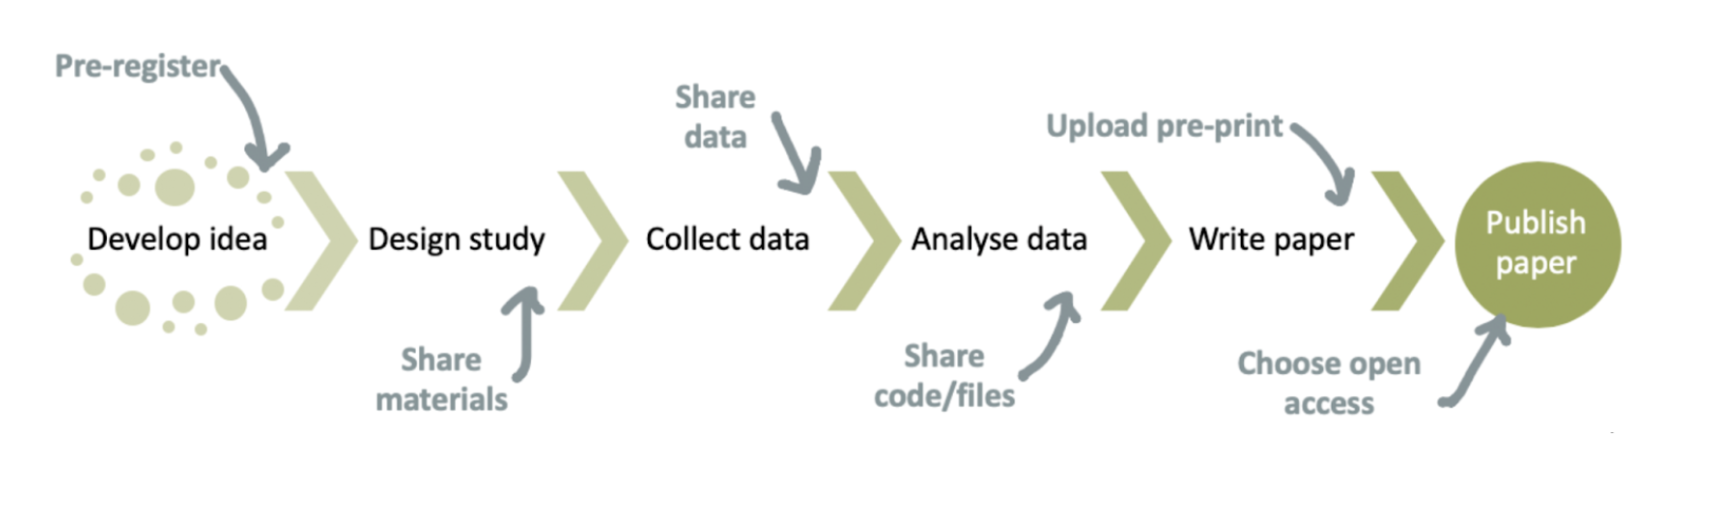
\includegraphics{workflow.png}

}

\caption{Source:
\url{https://jamesbrandscience.github.io/tutorials/open_science/Introduction.html\#1}}

\end{figure}

\bookmarksetup{startatroot}

\hypertarget{pre-registration-1}{%
\chapter*{1. Pre-Registration}\label{pre-registration-1}}
\addcontentsline{toc}{chapter}{1. Pre-Registration}

\markboth{1. Pre-Registration}{1. Pre-Registration}

\hypertarget{pre-registration-2}{%
\subsection*{\texorpdfstring{\textbf{Pre-registration}}{Pre-registration}}\label{pre-registration-2}}
\addcontentsline{toc}{subsection}{\textbf{Pre-registration}}

A preregistration is a document that outlines the plan for conducting
research before any data is collected or analyzed. This document, which
typically includes the introduction and methods sections of a research
paper, serves as a time-stamped record of the research plan. At a
minimum, a preregistration should include the hypotheses to be tested,
the methodology and variables that will be used (including the design,
sample, stopping rule, exclusion criteria, procedure, and variables),
the analysis plan (including statistical tests, transformations, and
assumption tests), and the criteria for inferring whether the hypotheses
have been confirmed or rejected.

\hypertarget{why-should-i-pre-register-my-research}{%
\subsection*{\texorpdfstring{\textbf{Why should I pre-register my
research?}}{Why should I pre-register my research?}}\label{why-should-i-pre-register-my-research}}
\addcontentsline{toc}{subsection}{\textbf{Why should I pre-register my
research?}}

There are several reasons why you should consider preregistering your
research:

\begin{itemize}
\item
  To clearly distinguish between confirmatory and exploratory analyses
  and avoid presenting exploratory results as if they were hypothesized.
\item
  To maintain transparency, preventing selective reporting and
  p-hacking.
\item
  To contribute to reducing the file drawer problem and publication
  bias.
\item
  To serve as a safety net for your future self: by preregistering your
  research, you won't have to rely on memory to recall your plans and
  methods. You'll only need to execute your plan (and report any
  deviations from it).
\item
  For more reasons to preregister, you may want to read
  \href{https://www.psychologicalscience.org/observer/seven-selfish-reasons-for-preregistration\#.WR3HblMrLOS}{this
  article}
\end{itemize}

\hypertarget{pre-registration-dilemmas}{%
\subsection*{\texorpdfstring{\textbf{Pre-registration
dilemmas}}{Pre-registration dilemmas}}\label{pre-registration-dilemmas}}
\addcontentsline{toc}{subsection}{\textbf{Pre-registration dilemmas}}

Preregistration can raise some dilemmas, but they are all easily
addressed:

\begin{itemize}
\item
  ``Preregistration costs too much time.'' The time you spend on
  preregistration is time you would normally spend after data
  collection. Preregistration can save you time because you won't waste
  time on pointless analyses; you've already written your introduction
  and methods sections.
\item
  ``What if my research doesn't go according to plan?'' You can add an
  addendum to your preregistration before the analysis to explain any
  deviations from the plan. Afterward, report any deviations in your
  manuscript. Transparency is the goal.
\item
  ``No one will ever look at my preregistration.'' You can use the
  preregistration as a reminder for yourself, as a justification to
  reviewers of your manuscript, and to inspire colleagues and interested
  researchers with your open attitude. Go for it!
\end{itemize}

\hypertarget{how-can-i-pre-register}{%
\subsection*{\texorpdfstring{\textbf{How can I
pre-register?}}{How can I pre-register?}}\label{how-can-i-pre-register}}
\addcontentsline{toc}{subsection}{\textbf{How can I pre-register?}}

See \href{https://osf.io/sgrk6/}{this link} for an easy tutorial on how
to preregister on the Open Science Framework (OSF). Don't forget to
include your collaborators and include the link to your preregistration
in your manuscript.

\hypertarget{what-are-registered-reports}{%
\subsection*{\texorpdfstring{\textbf{What are Registered
Reports?}}{What are Registered Reports?}}\label{what-are-registered-reports}}
\addcontentsline{toc}{subsection}{\textbf{What are Registered Reports?}}

Registered Reports are a type of preregistration that undergoes peer
review by journals. This greatly reduces publication bias because at
Stage 1 peer review, reviewers do not know the results, so manuscripts
cannot be accepted or rejected based on them. The process of Registered
Reports is shown below:

\begin{figure}

{\centering 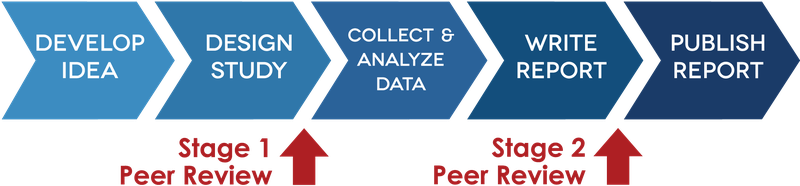
\includegraphics[width=6.25in,height=\textheight]{regreports.png}

}

\caption{Source:
\url{https://eur-synclab.github.io/open-science/preregistration.html}}

\end{figure}

After your preregistration has received an In Principle Acceptance
(Stage 1), you can start collecting data and writing up your results.
Most journals that get through Stage 1 will also get accepted in Stage
2, because the study design has already been reviewed.

\hypertarget{resources}{%
\section*{\texorpdfstring{\textbf{Resources}}{Resources}}\label{resources}}
\addcontentsline{toc}{section}{\textbf{Resources}}

\markright{\textbf{Resources}}

\begin{itemize}
\item
  All \href{https://osf.io/zab38/wiki/home/}{OSF templates}
\item
  A list of \href{https://www.cos.io/our-services/prereg}{resources on
  preregistration}
\item
  Information about
  \href{https://www.cos.io/our-services/registered-reports}{Registered
  Reports}
\item
  Overview of
  \href{https://docs.google.com/spreadsheets/d/1D4_k-8C_UENTRtbPzXfhjEyu3BfLxdOsn9j-otrO870/edit?usp=sharing}{all
  journals doing Registered Reports}
\item
  A preregistration tutorial and template for
  \href{https://psyarxiv.com/hvfmr}{secondary data analysis}
\item
  Preregistration: \href{https://psyarxiv.com/d8wex/}{dream vs.~reality}
\end{itemize}

\bookmarksetup{startatroot}

\hypertarget{data-management-plan-dmp}{%
\chapter*{2. Data Management Plan
(DMP)}\label{data-management-plan-dmp}}
\addcontentsline{toc}{chapter}{2. Data Management Plan (DMP)}

\markboth{2. Data Management Plan (DMP)}{2. Data Management Plan (DMP)}

\hypertarget{what-is-a-data-management-plan}{%
\subsection*{\texorpdfstring{\textbf{What is a Data Management
Plan?}}{What is a Data Management Plan?}}\label{what-is-a-data-management-plan}}
\addcontentsline{toc}{subsection}{\textbf{What is a Data Management
Plan?}}

A data management plan (DMP) is a document that outlines how data will
be collected, organized, stored, preserved, and shared during a research
project. A DMP is usually required by funding agencies, publishers, or
institutions as a way to ensure that research data are managed
appropriately and meet legal, ethical, and practical standards.

\hypertarget{what-are-the-main-components-of-a-dmp}{%
\subsection*{\texorpdfstring{\textbf{What are the main components of a
DMP?}}{What are the main components of a DMP?}}\label{what-are-the-main-components-of-a-dmp}}
\addcontentsline{toc}{subsection}{\textbf{What are the main components
of a DMP?}}

The main components of a DMP may include:

\begin{itemize}
\item
  Description of the data: What type of data will be collected or
  generated, and how will they be structured?
\item
  Data collection methods: How will the data be collected (e.g.,
  surveys, experiments, observations), and what tools or equipment will
  be used?
\item
  Data organization and documentation: How will the data be named,
  labeled, and organized to ensure consistency and usability?
\item
  Data storage and backup: Where and how will the data be stored (e.g.,
  local servers, cloud-based platforms), and how often will they be
  backed up?
\item
  Data sharing and reuse: Who will have access to the data, under what
  conditions, and for what purposes?
\item
  Data retention and preservation: How long will the data be kept, and
  how will they be preserved and made accessible after the end of the
  project?
\end{itemize}

\hypertarget{general-steps-to-write-a-dmp}{%
\subsection*{\texorpdfstring{\textbf{General steps to write a
DMP}}{General steps to write a DMP}}\label{general-steps-to-write-a-dmp}}
\addcontentsline{toc}{subsection}{\textbf{General steps to write a DMP}}

\begin{itemize}
\item
  Identify the key data types and formats you will collect or generate
  during your research project.
\item
  Determine how you will organize and store the data. Consider factors
  such as security, backup, and accessibility.
\item
  Decide how you will manage any ethical or legal issues related to your
  data. This may involve obtaining informed consent from participants,
  ensuring compliance with privacy regulations, or addressing
  intellectual property rights.
\item
  Establish guidelines for documenting your data. This may include
  creating metadata, labeling your files, and maintaining a data
  dictionary.
\item
  Develop a plan for sharing your data. Consider what data should be
  shared, with whom, and under what conditions.
\item
  Develop a plan for preserving your data after completing your project.
  Consider how long you will need to keep the data and how you will
  ensure that it remains accessible and usable.
\end{itemize}

Some funding agencies, institutions, or publishers may provide templates
or guidelines for writing a DMP. Additionally, there are several online
tools available, such as the \href{https://dmptool.org/}{DMPTool},
\href{https://www.dataone.org/}{DataOne}, or
\href{https://argos.openaire.eu/home}{Argos} that can help guide you
through the process of creating a DMP tailored to your specific needs.

When writing your DMP, it is important to be as specific as possible and
to consider all aspects of your data management strategy. Consult with
colleagues or data management experts if you need guidance or feedback.

\hypertarget{resources-1}{%
\section*{\texorpdfstring{\textbf{Resources}}{Resources}}\label{resources-1}}
\addcontentsline{toc}{section}{\textbf{Resources}}

\markright{\textbf{Resources}}

\begin{itemize}
\item
  More information about
  \href{https://www.uu.nl/en/research/research-data-management/guides/storing-and-preserving-data}{data
  management} (storing, archiving, versioning, data structure, etc.) and
  \href{https://www.openaire.eu/raw-data-backup-and-versioning}{backing
  up and versioning data}
\item
  How to \href{https://speakerdeck.com/jennybc/how-to-name-files}{name
  your files}
\item
  The
  \href{https://www.uu.nl/en/research/research-data-management/guides/costs-of-data-management}{costs
  of data management}
\item
  More about
  \href{https://www.eur.nl/en/library/research-support/research-data-management-rdm/privacy-and-legal-aspects}{privacy
  and legal aspects}
\item
  FCT
  \href{https://myfct.fct.pt/LibDocument/DocumentPatterns.FileDisplay.aspx?EcrypDoctId=omRid7suIkRYq\%2BIqLH1qkQ\%3D\%3D}{DMP
  template}
\item
  ERC
  \href{https://erc.europa.eu/sites/default/files/document/file/ERC-Data-Management-Plan.docx}{DMP
  template}
\end{itemize}

\bookmarksetup{startatroot}

\hypertarget{data-collection-protocols-1}{%
\chapter*{3. Data Collection
Protocols}\label{data-collection-protocols-1}}
\addcontentsline{toc}{chapter}{3. Data Collection Protocols}

\markboth{3. Data Collection Protocols}{3. Data Collection Protocols}

Soon available

\bookmarksetup{startatroot}

\hypertarget{data-dictionary-1}{%
\chapter*{4. Data Dictionary}\label{data-dictionary-1}}
\addcontentsline{toc}{chapter}{4. Data Dictionary}

\markboth{4. Data Dictionary}{4. Data Dictionary}

A data dictionary or a code book serves as a guide for interpreting the
metadata of your data files, explaining the meanings of variable names
and values. By providing clear documentation of your data, a codebook
can enhance the reproducibility of your research. It can be particularly
useful for facilitating collaborations and ensuring that you and others
can understand and use the data in the future. Additionally, if you
intend to share your datasets, creating a codebook is strongly
recommended.

Prior to embarking on the creation of a data dictionary, it may be
advisable to peruse this introductory guide on producing codebooks and
datasets that can be readily shared:

\href{https://osf.io/vd4y3/}{Buchanan, E. M., Crain, S. E., Cunningham,
A. L., Johnson, H. R., Stash, H. E., Papadatou-Pastou, M., \ldots{}
Aczel, B. (2019, May 20). Getting Started Creating Data Dictionaries:
How to Create a Shareable Dataset.
https://doi.org/10.31219/osf.io/vd4y3}

If you use R to analyze your data, you can use the
\href{https://rubenarslan.github.io/codebook/index.html}{codebook
package} to create a codebook based on the dataframe you are working
with.

\bookmarksetup{startatroot}

\hypertarget{logbook-1}{%
\chapter*{5. Logbook}\label{logbook-1}}
\addcontentsline{toc}{chapter}{5. Logbook}

\markboth{5. Logbook}{5. Logbook}

Soon available

\bookmarksetup{startatroot}

\hypertarget{data-storage-1}{%
\chapter*{6. Data Storage}\label{data-storage-1}}
\addcontentsline{toc}{chapter}{6. Data Storage}

\markboth{6. Data Storage}{6. Data Storage}

Soon available

\bookmarksetup{startatroot}

\hypertarget{scripts-1}{%
\chapter*{7. Scripts}\label{scripts-1}}
\addcontentsline{toc}{chapter}{7. Scripts}

\markboth{7. Scripts}{7. Scripts}

Sharing analysis code in research has several benefits, including:

\begin{itemize}
\item
  Reproducibility: Sharing code allows other researchers to replicate
  your analysis and verify your findings. This is important because
  reproducibility is a fundamental aspect of scientific research.
\item
  Transparency: Sharing code makes your research more transparent by
  allowing others to see exactly how you conducted your analysis. This
  helps to build trust in your results and allows others to build upon
  your work.
\item
  Efficiency: Sharing code can save other researchers time and effort by
  allowing them to build upon your work instead of starting from
  scratch. This can lead to more rapid progress in a field of study.
\item
  Collaboration: Sharing code can facilitate collaboration between
  researchers by allowing them to easily share their work and build upon
  each other's ideas.
\item
  Education: Sharing code can be a valuable educational resource for
  students and other researchers who are interested in learning new
  techniques or methods.
\end{itemize}

Overall, sharing analysis code in research can help to promote open
science and advance the progress of scientific research.

Web-based technologies make it very easy to share these materials (and
even to share the complete software environment using
\href{https://www.docker.com/}{Docker} and
\href{https://sylabs.io/singularity/}{Singularity} containers). However,
just releasing your code without annotation is not very informative
because others (and future you!) can't make a lot of sense of it. Two
helpful tools to annotate your code are RMarkdown and Jupyter notebooks.

R Markdown and Jupyter notebooks are tools that allow researchers to
create executable documents that combine code, text, and data. These
tools make research more reproducible in several ways:

\begin{itemize}
\item
  Documentation: R Markdown and Jupyter notebooks allow researchers to
  document their analysis in real-time, making it easier for others to
  understand the steps taken in the analysis.
\item
  Version control: These tools allow researchers to track changes to
  their analysis and code over time, making it easier to reproduce
  previous analyses and results.
\item
  Code sharing: R Markdown and Jupyter notebooks allow researchers to
  share their code and data with others, making it easier to reproduce
  their analysis.
\item
  Reproducibility: By combining code, text, and data in a single
  document, R Markdown and Jupyter notebooks make it easier for others
  to reproduce a researcher's analysis and results. This helps to ensure
  that research findings are accurate and reliable.
\item
  Collaboration: R Markdown and Jupyter notebooks make it easy for
  researchers to collaborate on an analysis, by allowing them to share
  and edit the same document.
\end{itemize}

\bookmarksetup{startatroot}

\hypertarget{metadata-1}{%
\chapter*{8. Metadata}\label{metadata-1}}
\addcontentsline{toc}{chapter}{8. Metadata}

\markboth{8. Metadata}{8. Metadata}

Metadata refers to data that describes other data. In other words, it's
information about the content, context, quality, and other
characteristics of a dataset. Metadata can include details such as the
dataset's title, author, date created, variable definitions, and data
format.

Metadata is crucial for achieving FAIR data, which stands for Findable,
Accessible, Interoperable, and Reusable. Without appropriate metadata,
it can be difficult or impossible to find, understand, or effectively
use a dataset. For example, if a researcher wants to locate data on a
particular topic, they may rely on metadata to search for and identify
relevant datasets. Similarly, metadata can help ensure that data are
properly documented, formatted, and described, facilitating their use by
other researchers. Metadata plays a critical role in enhancing the
discoverability, usability, and overall value of research data.

\hypertarget{examples-of-research-metadata}{%
\subsection*{\texorpdfstring{\textbf{Examples of research
metadata}}{Examples of research metadata}}\label{examples-of-research-metadata}}
\addcontentsline{toc}{subsection}{\textbf{Examples of research
metadata}}

\begin{itemize}
\item
  A project readme containing the information below. Often in a
  readme.txt. Find an example
  \href{https://cornell.app.box.com/v/ReadmeTemplate}{template here} or
  use the information below:

  \begin{itemize}
  \item
    Creator (PI): name and affiliation of PI
  \item
    Title: project title
  \item
    Funding sources: names of funders, incl.~grant numbers and related
    acknowledgements
  \item
    Data collector/producer: who is responsible for data collection +
    date and location of data production
  \item
    Description: project description, incl.~relevant publications
  \item
    Sample and sampling procedures: target population and methods to
    sample it (or link to document describing this), retention rates for
    longitudinal studies
  \item
    Coverage: topics, time period and location covered
  \item
    Source: if relevant, citations to original source from which data
    were obtained
  \end{itemize}
\item
  Metadata for a specific data file, containing, for example, file
  description, data format, relationship with other files, date of
  creation and versioning information, etc. This can be a readme.txt or
  other filetypes, such as nameofdatafile.json or nameofdatafile.xml
\item
  A codebook (data dictionary), which specifies what all variables in
  your dataset mean. See \protect\hyperlink{data-dictionary-1}{Data
  Dictionary} for more information.

  \begin{itemize}
  \item
    Question wording or meaning
  \item
    Variable text: question text or item number
  \item
    Respondent: who was asked the question?
  \item
    Meaning of codes: interpretation of the codes assigned to each
    variable
  \item
    Missing data codes, e.g., 999
  \item
    Summary statistics for both valid and missing cases
  \item
    Imputation and editing: identify data that have been estimated or
    extensively edited
  \item
    Constructed and weight variables: how were they constructed
  \item
    Location in the data file: field or column location, if relevant
  \item
    Variable groupings: if you categorize variables into conceptual
    groupings
  \end{itemize}
\item
  Metadata in systems, such as a data repository. This type of metadata
  is often enforced and interoperable so that you don't have to manually
  create this type of metadata.
\end{itemize}

\hypertarget{metadata-standards}{%
\subsection*{\texorpdfstring{\textbf{Metadata
standards}}{Metadata standards}}\label{metadata-standards}}
\addcontentsline{toc}{subsection}{\textbf{Metadata standards}}

Metadata standards refer to the frameworks that provide guidelines for
the metadata fields, defining the formatting of metadata fields to make
them machine-readable and interoperable. An extensive range of metadata
standards is available, varying across different disciplines. For the
social sciences, the most widely known metadata standards are
\href{https://www.dublincore.org/}{Dublin Core} and
\href{https://ddialliance.org/}{Data Documentation Initiative} (DDI).
Dublin Core consists of basic elements for describing networked
resources, such as Title, Creator, Subject, Description, Publisher,
Contributor, Date, Type, Format, and Identifier, among others (check
this
\href{https://nsteffel.github.io/dublin_core_generator/generator_nq.html}{metadata
file generator} to see all the elements). On the other hand, DDI is
commonly used in social, behavioral, economic, and health sciences,
including \href{https://www.cessda.eu/}{CESSDA} (Consortium of European
Social Science Data Archives). Researchers may not always need to work
directly with these standards, but it is important to understand that
different repositories may adopt different standards. More metadata
standards can be found
\href{https://zenodo.org/record/3543756\#.ZAkCnuxUmrO}{here}.

\bookmarksetup{startatroot}

\hypertarget{version-control-1}{%
\chapter*{9. Version Control}\label{version-control-1}}
\addcontentsline{toc}{chapter}{9. Version Control}

\markboth{9. Version Control}{9. Version Control}

Version control of files is the practice of tracking changes made to a
file over time, creating a history of revisions that can be reviewed,
reverted, or compared. It involves using specialized software tools that
allow users to manage and store different versions of a file, along with
associated metadata such as timestamps, authorship, and comments.

Version control is commonly used in software development to manage the
source code of a project, but it can also be applied to any type of
file, including text documents, spreadsheets, graphics, and multimedia
files. By keeping different versions of a file separated and organized,
version control helps to avoid data loss, reduce errors, and enable
collaboration among multiple users working on the same file.

It is highly recommended to make a habit out of at least one, but
preferably more of the following practices if you do not (want to) use a
formal version control system:

\begin{itemize}
\item
  Keep raw data separately from any processed data and document which
  steps have been taken to go from the former to the latter
\item
  Rename a file every time you make a sizable change
\item
  Use dates in the filename in the format YYYYMMDD
\item
  Append the filename with a version number, e.g., document\_v1.0,
  document\_v1.2, etc.
\item
  See \href{https://authors.library.caltech.edu/103626/}{this link} for
  a helper document for coming up with a good file naming convention
\item
  Include a versioning history within the document, e.g., on the first
  page, explaining what changed in which version
\item
  Use services like Google drive and Dropbox, which allow collaborative
  editing but also reverting to previous versions
\end{itemize}

\hypertarget{formal-version-control-systems}{%
\subsection*{\texorpdfstring{\textbf{Formal Version Control
Systems}}{Formal Version Control Systems}}\label{formal-version-control-systems}}
\addcontentsline{toc}{subsection}{\textbf{Formal Version Control
Systems}}

Formal version control systems are software tools that are designed to
help manage changes to files, particularly source code files in software
development projects. They enable users to track modifications made to a
file over time, store different versions of the file, and collaborate
with other users. Formal version control systems typically provide
features such as:

\begin{itemize}
\item
  Check-in and check-out of files
\item
  Version history tracking
\item
  Branching and merging of files
\item
  Access control and permission management
\item
  Annotation and commenting on changes
\item
  Diff and merge tools for comparing versions
\item
  Integration with other development tools and platforms
\end{itemize}

Examples of formal version control systems include Git, Subversion
(SVN), Mercurial, and Perforce. These systems are widely used in
software development teams and other collaborative projects where file
versioning, change tracking, and collaboration are critical.

\bookmarksetup{startatroot}

\hypertarget{preprints-1}{%
\chapter*{10. Preprints}\label{preprints-1}}
\addcontentsline{toc}{chapter}{10. Preprints}

\markboth{10. Preprints}{10. Preprints}

Preprints are early versions of research papers that have not yet
undergone peer review or been published in a scientific or academic
journal. They are typically posted on preprint servers, which are online
repositories that allow authors to share their work with the wider
research community before publication.

Preprints often contain preliminary results or research findings that
are still being refined or validated. They are intended to facilitate
the dissemination of research findings and enable early feedback and
collaboration among researchers.

Preprints are becoming increasingly popular in many scientific
disciplines, including physics, biology, computer science, and
archaeology. They offer several benefits, such as faster dissemination
of research, increased collaboration opportunities, and the ability to
receive feedback from a wider range of experts in the field.

See more info in this
\href{https://help.osf.io/article/230-preprint-faqs}{Preprint FAQ}

\hypertarget{why-publish-preprints}{%
\subsection*{\texorpdfstring{\textbf{Why publish
preprints?}}{Why publish preprints?}}\label{why-publish-preprints}}
\addcontentsline{toc}{subsection}{\textbf{Why publish preprints?}}

There are several reasons why researchers choose to publish preprints:

\begin{itemize}
\item
  Rapid dissemination of research findings: Preprints enable researchers
  to share their work quickly and easily with the wider scientific
  community, leading to more rapid dissemination of research findings.
\item
  Increased visibility and impact: By making their research available as
  a preprint, researchers can increase the visibility and impact of
  their work, as it can be accessed and cited by other researchers
  before it is formally published.
\item
  Early feedback and collaboration: Preprints allow researchers to
  receive early feedback and engage in collaborative discussions with
  other experts in their field, which can help to improve the quality of
  their research.
\item
  Avoidance of long review processes: Formal peer review can be a
  lengthy and time-consuming process. Publishing preprints can reduce
  the time from submission to publication, as it enables researchers to
  receive feedback and make revisions before submitting their work to a
  journal.
\item
  Open science and transparency: Publishing preprints is part of a
  growing movement towards open science and transparency in research,
  which aims to make scientific findings more accessible to the public
  and increase trust in scientific research.
\end{itemize}

\hypertarget{where-to-publish-preprints}{%
\subsection*{\texorpdfstring{\textbf{Where to publish
preprints?}}{Where to publish preprints?}}\label{where-to-publish-preprints}}
\addcontentsline{toc}{subsection}{\textbf{Where to publish preprints?}}

Preferably a preprint server that provides a persistent identifier. For
example:

\begin{itemize}
\item
  \href{https://osf.io/preprints/}{OSF Preprints}: you can choose many
  preprint servers and can also share supplementary files. A list of
  preprint servers hosted via OSF Preprints can be found
  \href{https://osf.io/preprints/discover?subject=bepress\%7CSocial\%20and\%20Behavioral\%20Sciences}{here}.
\item
  Directly via a preprint server, such as
  \href{https://www.biorxiv.org/}{BioRxiv} or
  \href{https://psyarxiv.com/}{PsyArXiv}
\item
  You can even add a preprint on
  \href{https://explore.researchgate.net/display/support/Preprints}{ResearchGate}!
\end{itemize}

\hypertarget{feedback-and-updating}{%
\subsection*{\texorpdfstring{\textbf{Feedback and
updating}}{Feedback and updating}}\label{feedback-and-updating}}
\addcontentsline{toc}{subsection}{\textbf{Feedback and updating}}

Researchers can give/receive feedback on preprints in different ways: -
In OSF preprints, you can use their tool Hypothes.is to annotate
preprints, see their
\href{https://help.osf.io/hc/en-us/articles/360019738554-annotate-a-preprint}{help
guide}.

What you do with feedback is completely up to you. If you want, you can
update your preprint to a new version. However, note that all versions
are timestamped and retained. Often new versions get a new identifier
(DOI) and old versions cannot be removed. If your work gets published by
a publisher, many preprint servers also offer the possibility to refer
to the identifier (DOI) of your published work, so that readers of the
preprint get a notification that they are not reading the most
up-to-date version.

\bookmarksetup{startatroot}

\hypertarget{peer-review-1}{%
\chapter*{11. Peer review}\label{peer-review-1}}
\addcontentsline{toc}{chapter}{11. Peer review}

\markboth{11. Peer review}{11. Peer review}

Soon available

\bookmarksetup{startatroot}

\hypertarget{references}{%
\chapter*{References}\label{references}}
\addcontentsline{toc}{chapter}{References}

\markboth{References}{References}

\hypertarget{refs}{}
\begin{CSLReferences}{0}{0}
\end{CSLReferences}



\end{document}
